\documentclass{article}
\usepackage[utf8]{inputenc}
\usepackage{graphicx}
\setlength{\parindent}{0pt}
\setlength{\parskip}{1em}

\title{FOAR705 - Learning Journal Week 4}
\author{Jan Jugueta - 44828020}
\date{Week 4: 19/8/19 - 25/8/19}

\begin{document}

\maketitle

\section*{19/8/19 - 11:50am}

New week. Time to upload and commit the Week 2 Learning Journal to Cloudstor and GitHub.

\textbf{Objective:} Upload and commit Week 2 Learning Journal to Cloudstor and GitHub.

\textbf{Action:} 
\begin{itemize}
    \item Downloaded Learning\_Journal\_Week\_3.pdf from Overleaf.
    \item Downloaded LearningJournalWeek3 folder from Overleaf, which includes the .tex file and two .png images.
    \item Created Week3 Folder in 2019-FOAR705-Collaboration/Journals/JuguetaLearningJournal.
    \item Uploaded JuguetaLJWeek3.tex, figa.png and figb.png to Cloudstor.
    \item Uploaded Learning\_Journal\_Week\_3.pdf to Cloudstor.
\end{itemize}

\textbf{Error:} None.

\textbf{Result:} Successfully uploaded and committed Learning Journal Week 3 to Cloudstor and GitHub.

\section*{19/8/19 - 12:09pm}

\textbf{Objective:} Upload edited SAFI\_dates.xlsx file from the Dates as Data exercise.

\textbf{Action:} 
\begin{itemize}
    \item Uploaded SAFI\_dates.xlsx file
    \item Committed file.
\end{itemize}

\textbf{Error:} None.

\textbf{Result:} Committed SAFI\_dates.xlsx file to GitHub.

\section*{19/8/19 - 12:14pm}

Continuing on with the \textbf{Data Carpentry} exercises. Currently going through the Quality Assurance lesson.

\textbf{Objective:} Complete ‘Restricting data to a numeric range’ section.

\textbf{Action:}
\begin{itemize}
    \item Opened SAFI\_clean.xlsx on Excel.
    \item Selected the no\_membrs column.
    \item Clicked on Data - Validation in the menu.
    \item Selected Whole Number from the Allow drop down menu.
    \item Entered 1 as the Minimum and 30 as the Maximum then clicked OK.
    \item Entered the 50 in cell D133.
    \item Went back to the Validation window.
    \item Changed the Input Message Title to ‘Invalid Number’ with the message ‘Please enter a number ranging from 1 to 30.’
\end{itemize}

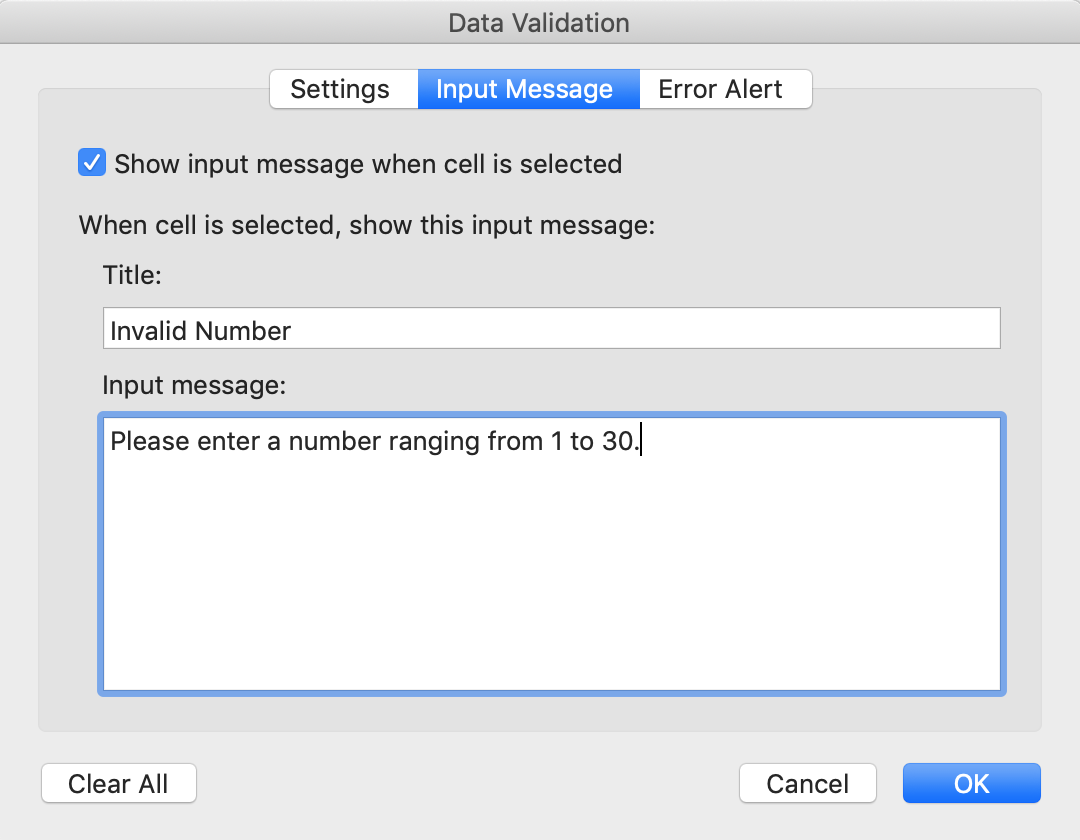
\includegraphics[width=\textwidth]{figa.png}

\textbf{Error:} Error: Only when entering the value 50 in cell D133 as instructed by the lesson.

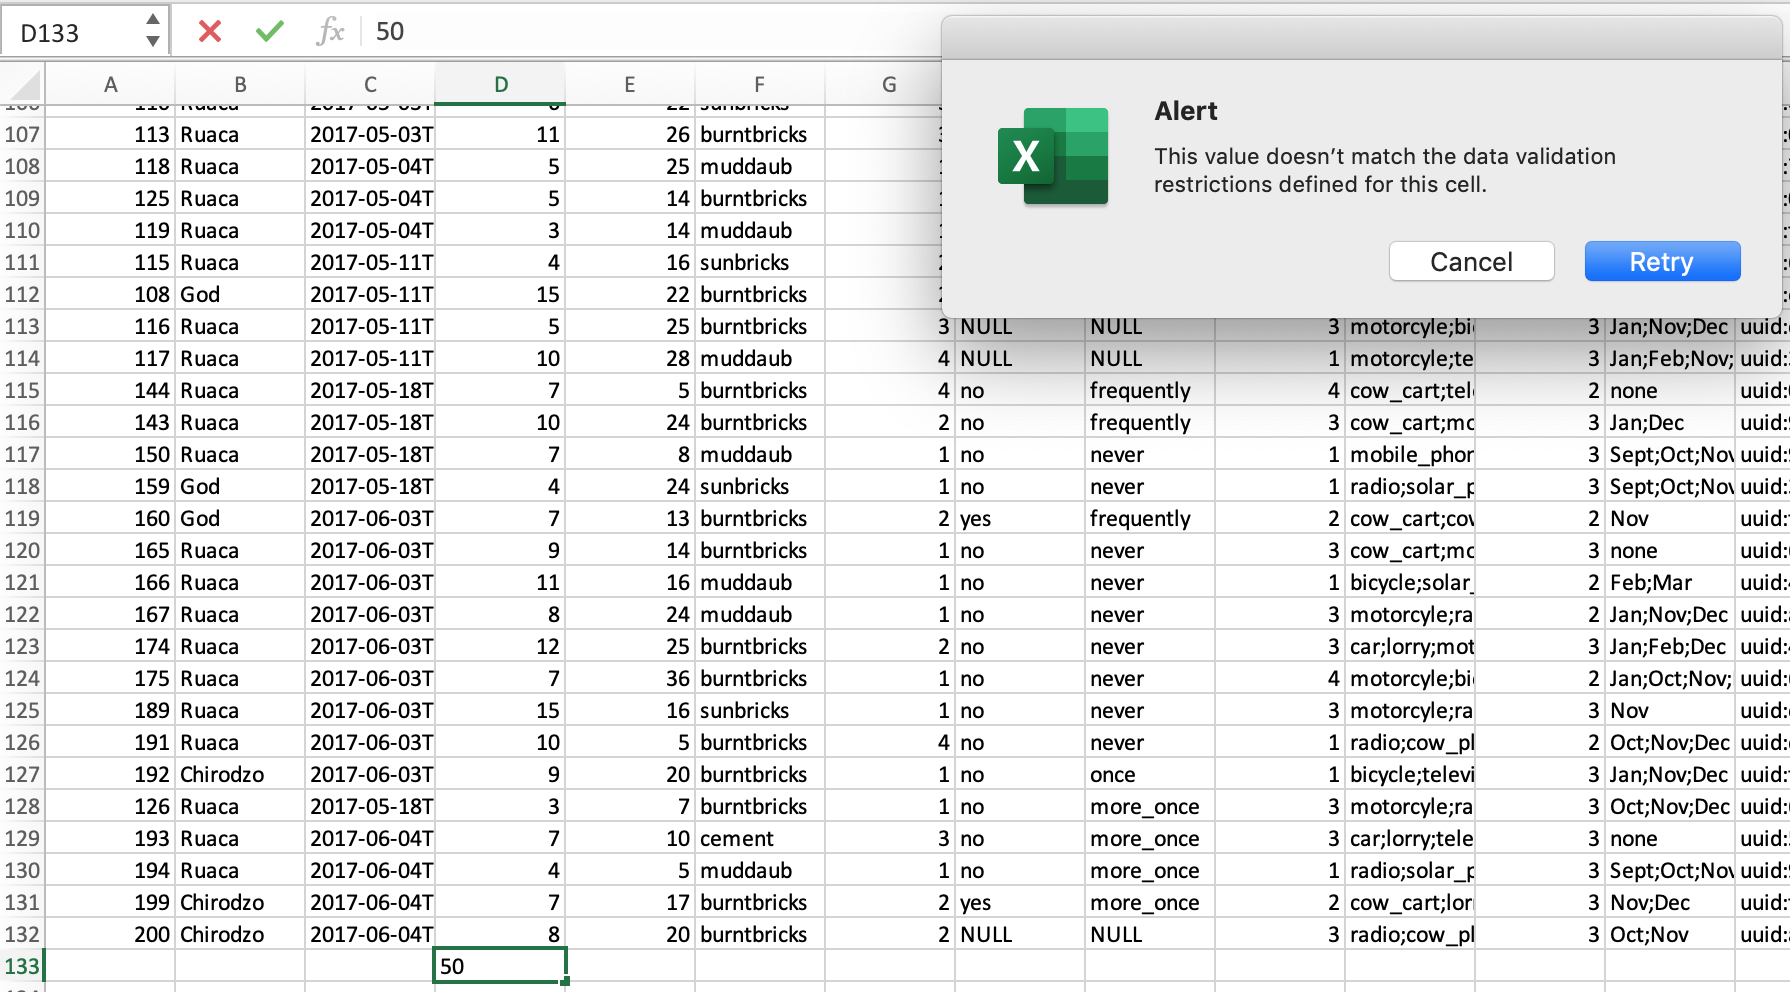
\includegraphics[width=\textwidth]{figb.png}

\textbf{Result:} Completed this section of the exercise. I now know how to restrict data entry and change the input message.

\section*{19/8/19 - 12:26pm}

Going on with the exercise, I will now try the Validation with another column in SAFI\_clean.xlsx.

\textbf{Objective:} Restrict data entry for the rooms column for values between 1 and 15.

\textbf{Action:} 
\begin{itemize}
    \item Select rooms column.
    \item Opened the Validation window.
    \item Allowed - Whole Numbers
    \item Inputted 1 for Minimum and 15 for Maximum.
    \item Changed Input Message Title to ‘Invalid Number’.
    \item Changed messaged to ‘Number must range from 1 to 15’.
    \item Tested validation by entering 16 into cell G133.
    \item Tested validation by entering 15 into cell G133.
\end{itemize}

\textbf{Error:} Error message occurred when entering 16 into G133.

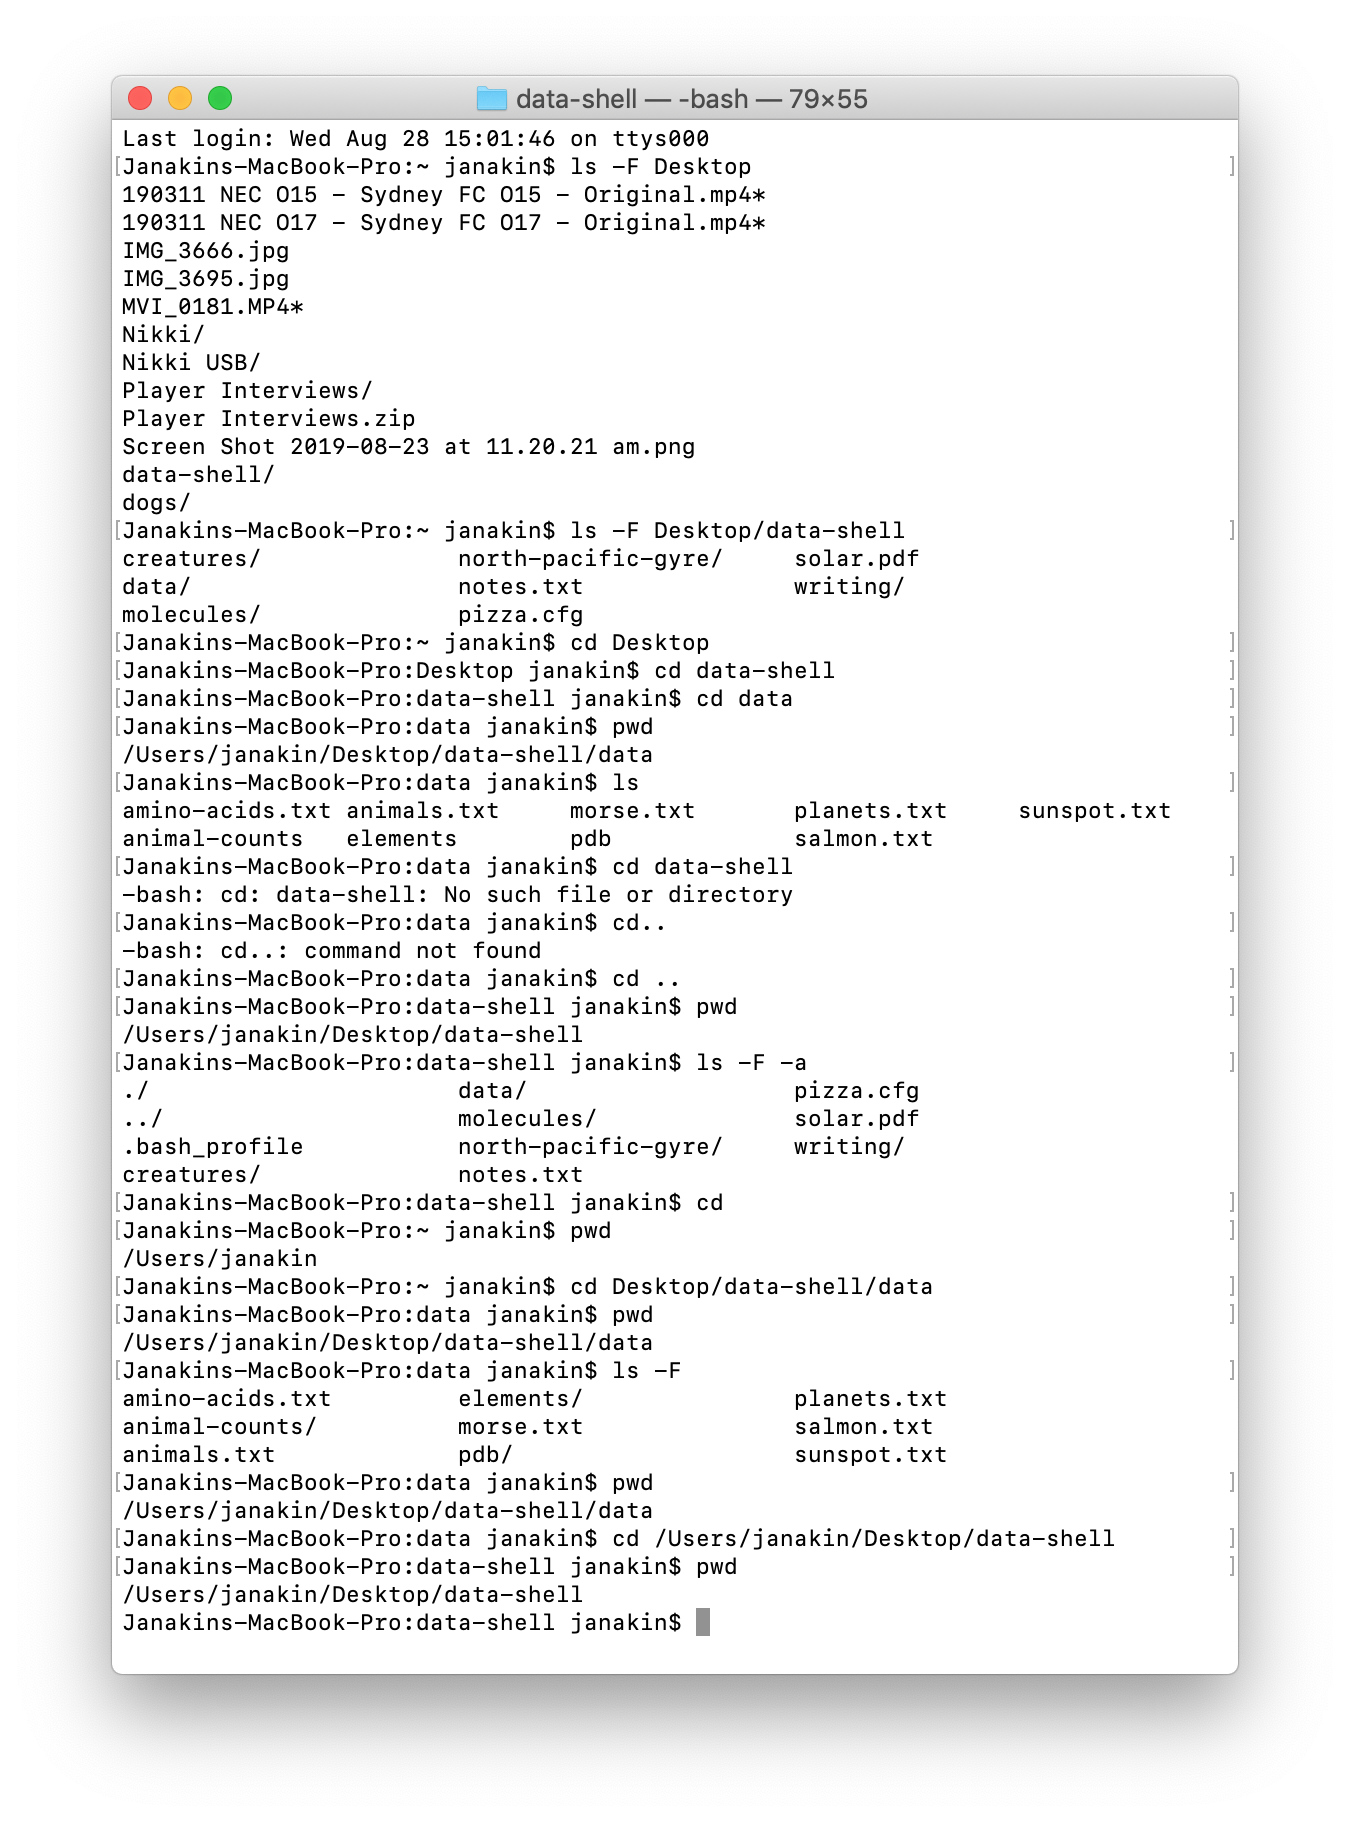
\includegraphics[width=\textwidth]{figc.png}

\textbf{Result:} Validation success.

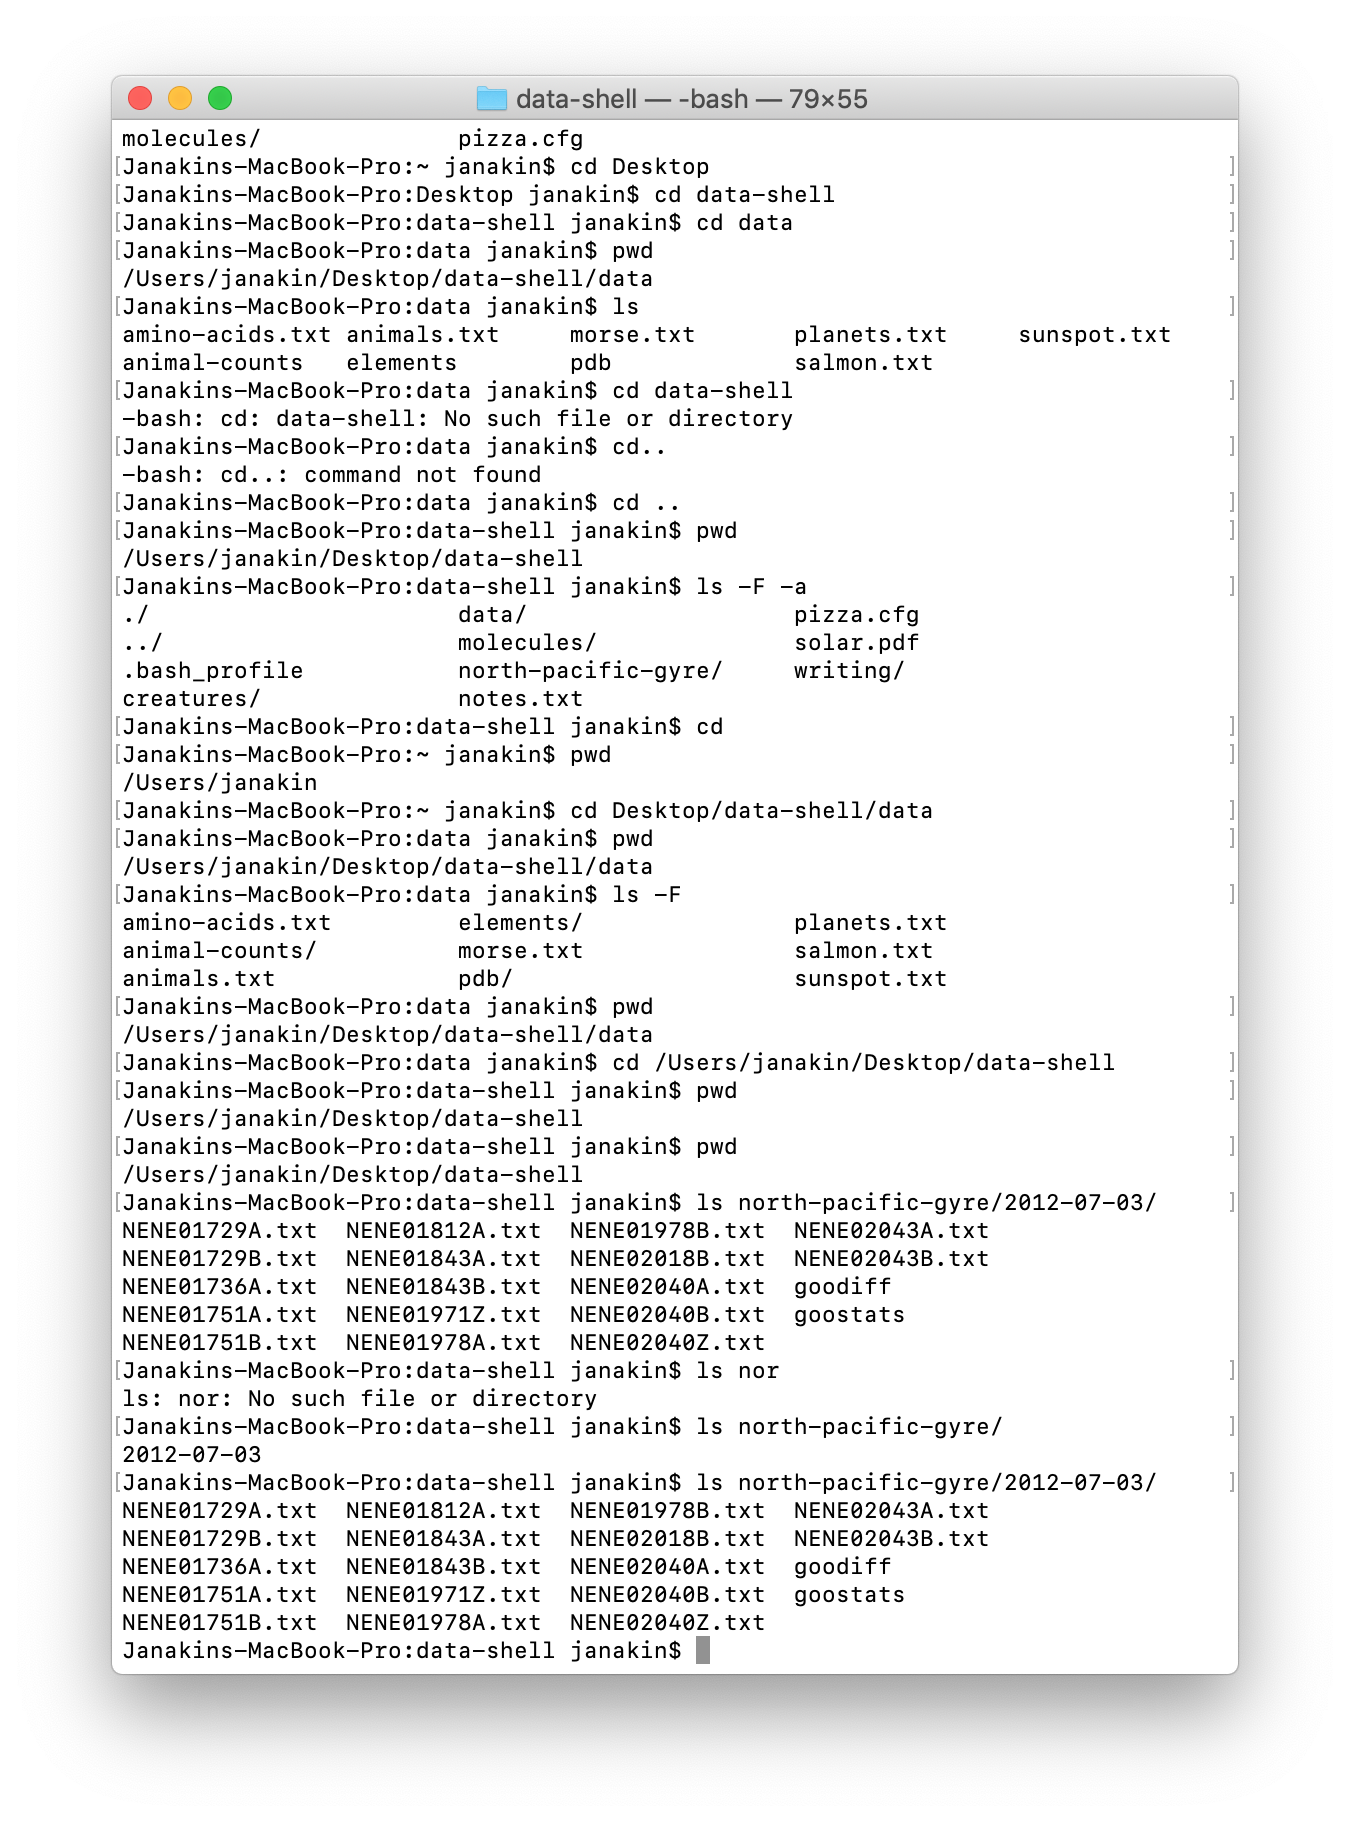
\includegraphics[width=\textwidth]{figd.png}

\section*{19/8/19 - 12:44pm}

Will now do the ‘Restricting data to entries from a list’ section.

\textbf{Objective:} Complete ‘Restricting data to entries from a list’ section.

\textbf{Action:}
\begin{itemize}
    \item Selected respondent\_wall\_type column.
    \item Opened the Validation window.
    \item Selected List from the Allow drop down menu in the Settings tab.
    \item Entered ‘grass, muddaub, burntbricks, sunbricks, cement’ into the source.
    \item Entered ‘Only selected items’ for the Input Message Title.
    \item Entered ‘grass, uddaub, burntbricks, sunbricks, cement’ for the Input Message.
    \item Clicked OK.
\end{itemize}

\textbf{Error:} None.

\textbf{Result:} Successfully restricted data entry from a list.

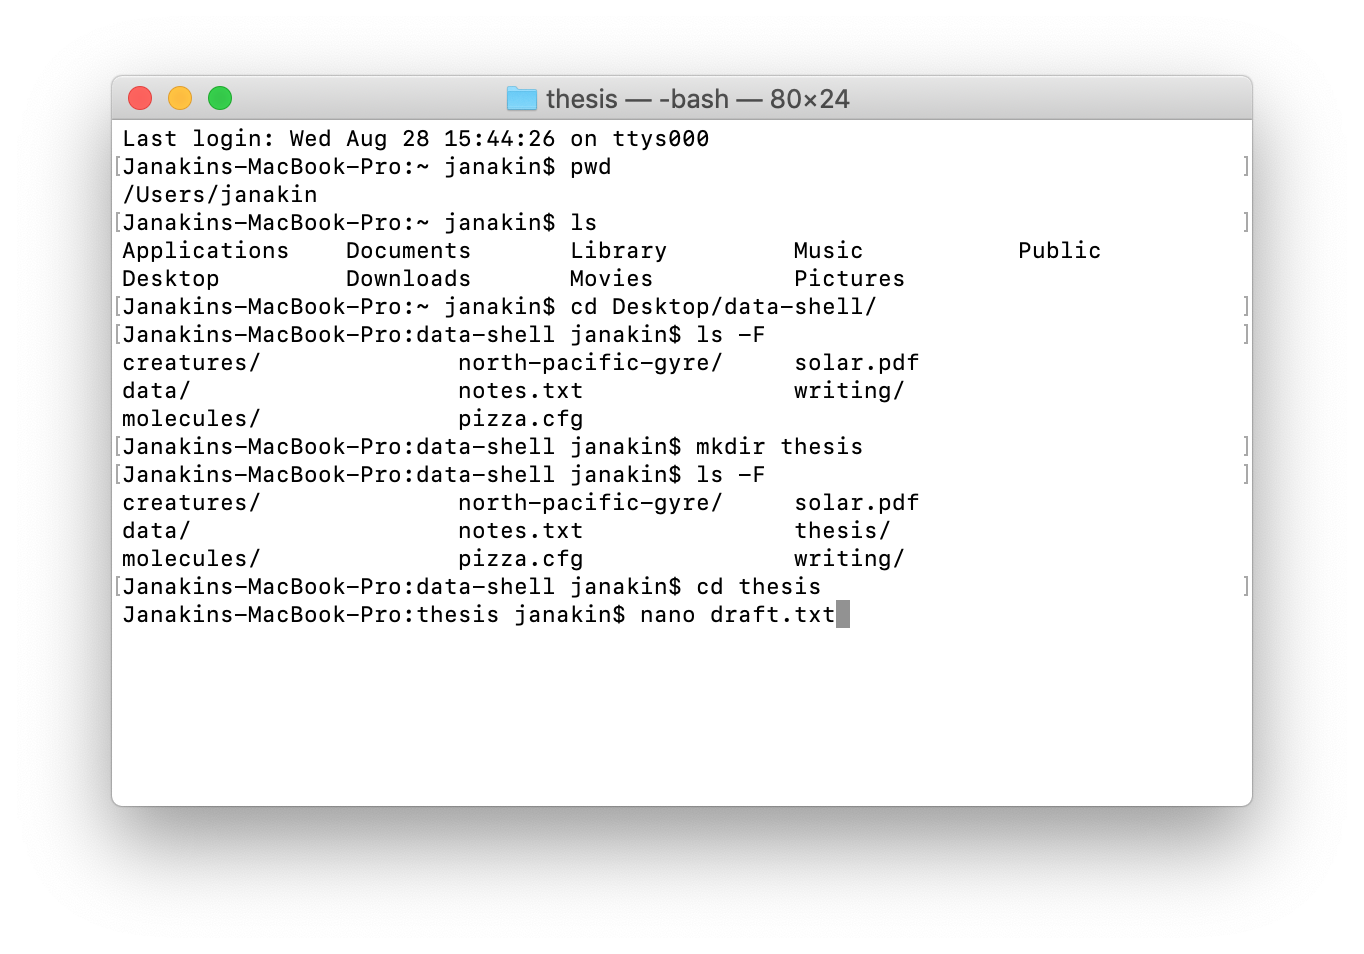
\includegraphics[width=\textwidth]{fige.png}

\section*{19/8/19 - 12:52pm}

Now to test the validation.

\textbf{Objective:} Test validation by entering an item not on the list.

\textbf{Action:}
\begin{itemize}
    \item Entered ‘steel’ in cell F133.
    \item Entered muddaub in cell F134.
\end{itemize}

\textbf{Error:} Only when entering ‘steel’ into F133.

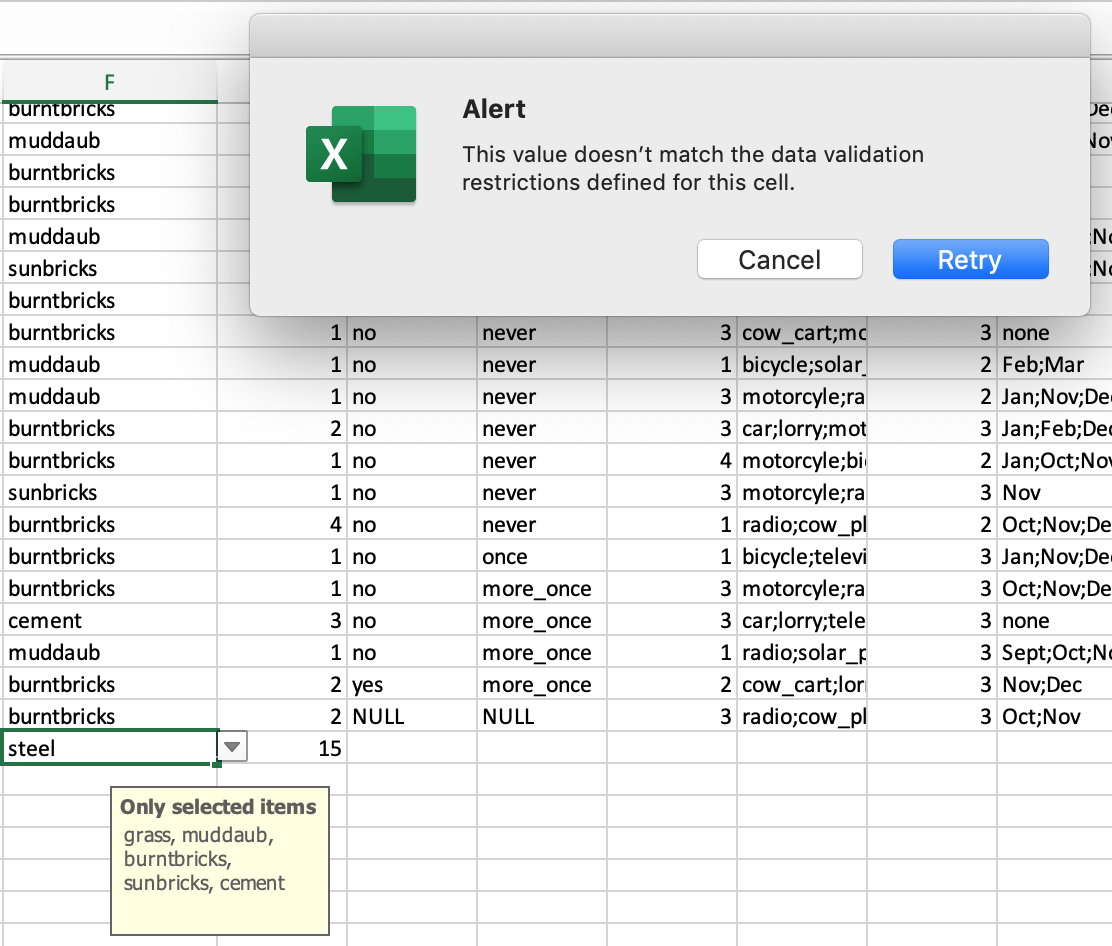
\includegraphics[width=\textwidth]{figf.png}

\textbf{Result:} Steel was not accepted, but muddaub was.

\section*{19/8/19 - 12:56pm}

Now I will try to restrict entry to a list for another column.

\textbf{Objective:} Restrict entry for column memb\_assoc to only yes, no or NULL.

\textbf{Action:}
\begin{itemize}
    \item Selected memb\_assoc column.
    \item Opened validation window.
    \item Selected List from the Allow drop down menu.
    \item Entered yes, no, NULL to the source.
    \item Entered ‘Only these items are allowed’ for Input Message Title and ‘yes, no, NULL’ to Input Message.
    \item Tested validation by entering ‘maybe’ to cell H133.
    \item Tested valdiation by entering yes to cell H134.
\end{itemize}

\textbf{Error:} Only when entering ‘maybe’ to cell H133.

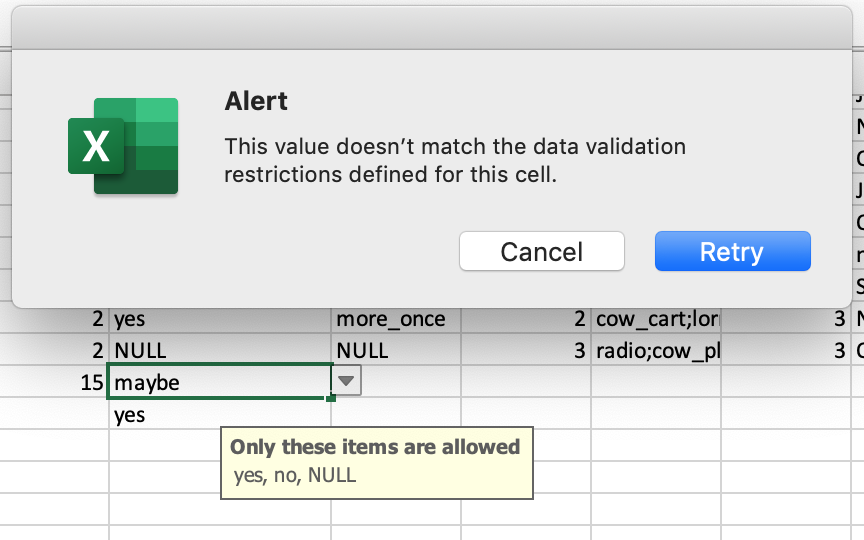
\includegraphics[width=\textwidth]{figg.png}

\textbf{Result:} Validation success. Only yes, no or NULL can be entered in the memb\_assoc column.

\section*{19/8/19 - 1:08pm}

Just finished reading the Exporting data lesson in Data Carpentry. The big takeaway point is that you should save your data in files that are universal and open. Which means saving data in .xlsx files isn’t a great idea. Instead, use files like .tsv or .csv.

\section*{19/8/19 - 1:09pm}

\textbf{Objective:} Save SAFI\_clean.xlsx as SAFI\_clean.csv

\textbf{Action:}
\begin{itemize}
    \item Clicked on File then Save As.
    \item Selected CSV as the file format.
    \item Renamed file SAFI\_clean\_edit.csv because there is an existent SAFI\_clean.csv file.
    \item Clicked save.
\end{itemize}

\textbf{Error:} None.

\textbf{Result:} Success. Data saved in new SAFI\_clean\_edit.csv file. 

\section*{19/8/19 - 1:12pm}

\textbf{Objective:} Commit SAFI\_clean\_edit.csv to GitHub.

\textbf{Action:}
\begin{itemize}
    \item Uploaded SAFI\_clean\_edit.csv
    \item Added description ‘SAFI\_clean\_edit.csv file from Data Carpentry’
    \item Added extended description ‘This commit contains a file that was made as part of the Data Carpentry Data Organization in Spreadsheets for Social Scientists. It contains work done as part of sections 4, 5 and 6.’
    \item Selected on Commit changes.
\end{itemize}

\textbf{Error:} None.

\textbf{Result:} Successfully committed SAFI\_clean\_edit.csv to GitHub.

\section*{22/8/19 - 2:11pm}

I have previously contacted some people from the FOAR705 class about the potential to collaborate on the Proof of Concept. I found some similarity with both Isaac Harrison and Lauren Franks (whom both have been in previous classes with me) in a potential project. We all tried to meet at a time convenient to us all, but unfortunately Lauren didn’t have a time that suited both Isaac and I. So I met with Isaac after another of our classes to discuss Scoping Exercise II. 

We identified that we had similar pains in relation to time management and note management. The following were the notes that we had come up with in our meeting.

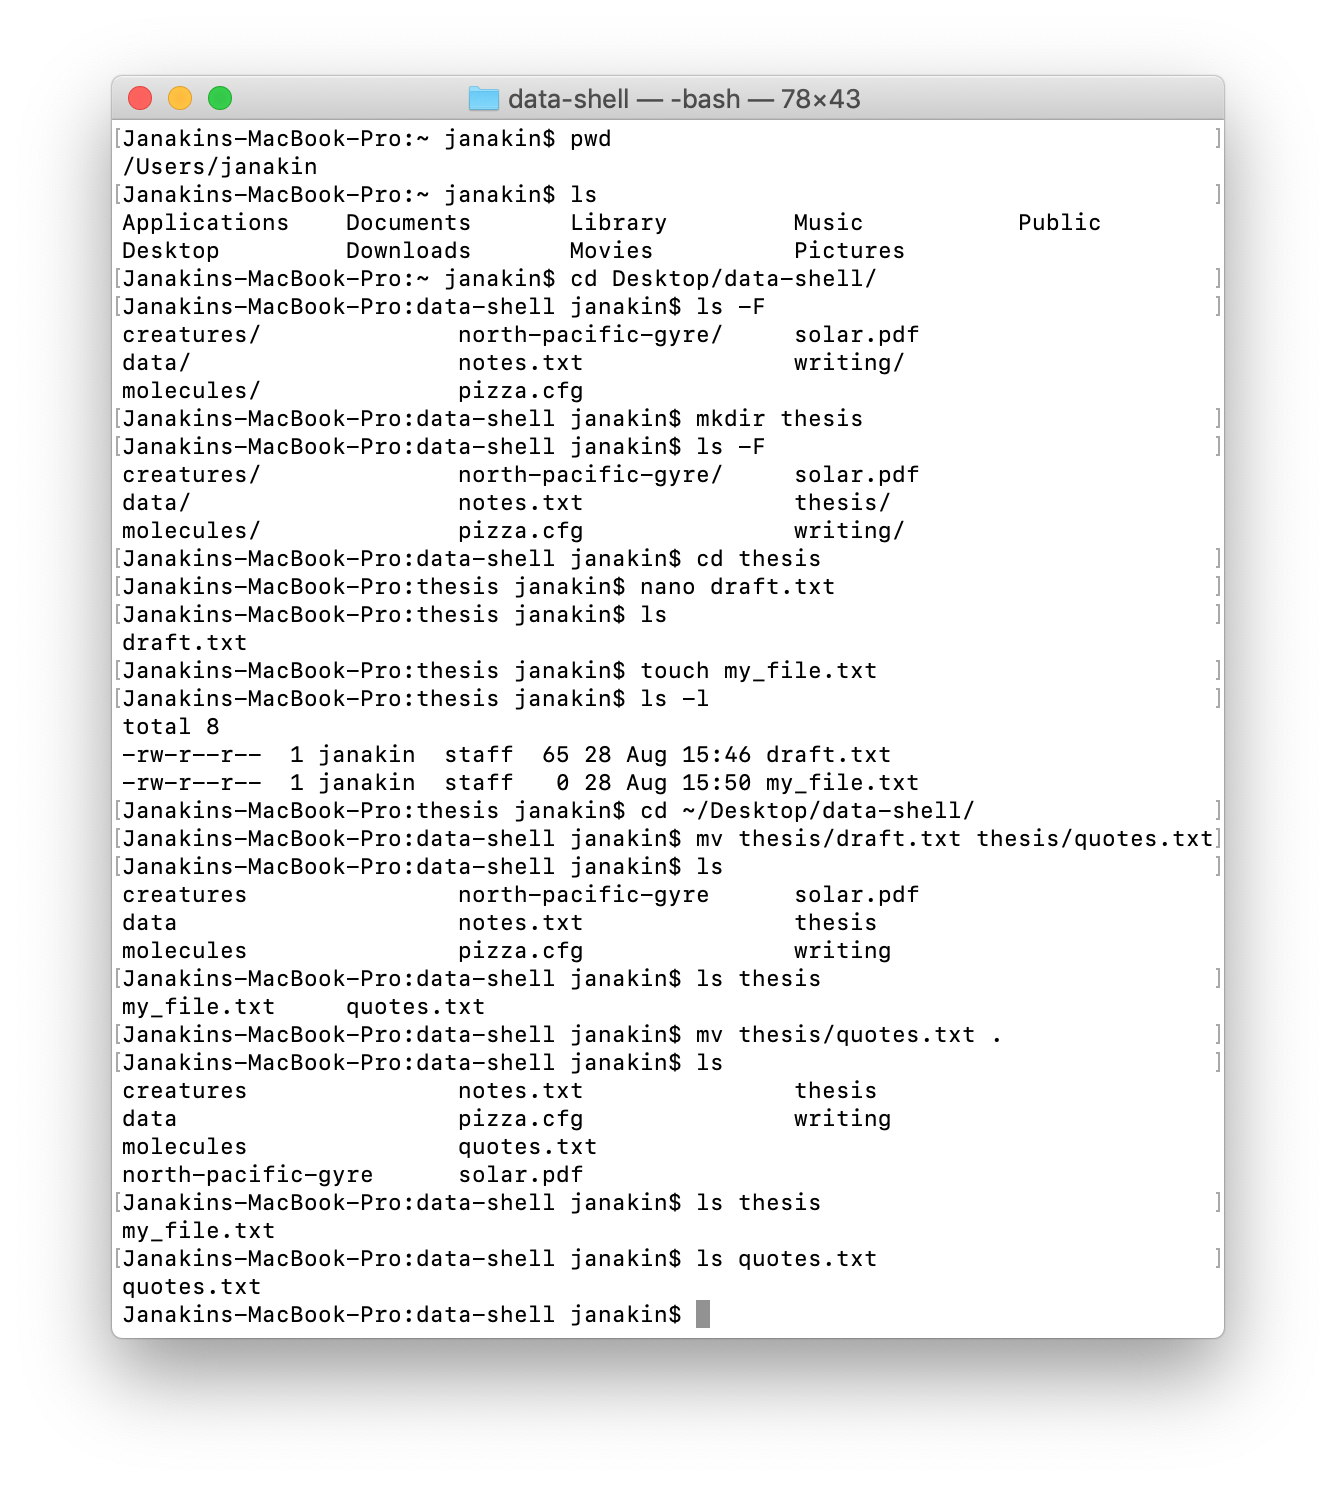
\includegraphics[width=\textwidth]{figh.png}

\end{document}
